\section{Method}
\label{sec:method}

\subsection{개요: 먼저 빼고, 필요하면 넣는다}
\label{sec:overview}
사용자가 자연어 과제를 주면 로봇은 머리 카메라와 손목 카메라 영상, 고유 감각(관절 위치, 그리퍼 폭, 전류)을 받아 팔 관절 명령을 낸다. 목표는 처음 보는 장면에서도 과제를 끝내는 것이고, 그다음이 빠르게 끝내는 것이다. PaceNotes는 층을 미리 쌓지 않는다. 먼저 가장 단순한 구성으로 과제가 되는지 확인하고, 빠진 부품 때문에 실제로 문제가 확인될 때만 그 부품을 넣는다(\cref{fig:teaser}).
\begin{itemize}
  \item \textbf{1단계(지금): 코드라이버가 직접 몬다.} 상위 계획기가 앞 구간을 읽고 움직임까지 지시하며, 단순한 결정적 실행기가 그 지시를 그대로 수행한다(\cref{sec:upper}). 상위 계획기를 학습 가능한 크기로 다듬고(\cref{sec:training}), 어디서 무너지는지 한계를 잰다(\cref{sec:plan}).
  \item \textbf{2단계(한계가 확인될 때만): 드라이버를 태운다.} 기다림 때문에 실패하거나 너무 느린 것처럼 1단계의 한계가 측정으로 확인되면, 실시간 세부 조종을 맡는 VLA 층을 붙인다. 두 모델은 원래 형식을 그대로 쓰고, 코드가 상위 목표를 매 틱 VLA 결정으로 바꿔 VLA 자신의 결정과 늘 섞는다(\cref{sec:extension}). 이 층은 구현과 일부 검증을 거쳤지만 지금은 보류해 둔다.
\end{itemize}
이 논문에서 쓰는 용어는 여섯이다. \textbf{상위 계획기}는 과제를 이해하고 구간 의도를 선언하며 결과를 검증하는 모델이다. 지금은 Astra(effort low)이고, 목표는 학습 가능한 크기의 오픈 VLM이다. \textbf{실행기}는 상위의 명령을 최소 저크 직선 운동으로 수행하는 코드다. \textbf{구간 의도}는 상위가 매 답의 진행 평가에 싣는 끝낸 일·지금 하는 일·남은 일과, 명령에 붙는 그리퍼 의도(잡을 것, 놓을 것)다. \textbf{검증}은 상위가 실행 결과를 보고 성공 여부(잡았다, 놓았다)를 판정하는 일이며, 확정 근거는 고유 감각 코드(T1)다. 2단계에서만 쓰는 용어가 둘 더 있다. \textbf{VLA}는 0.33\,s마다 typed 결정을 고르는 빠른 모델이고, \textbf{행동 전문가}는 확정된 결정을 0.4\,s 관절 청크로 바꾸는 흐름 정합 모듈이다.

\subsection{1단계: 상위 계획기와 실행기}
\label{sec:upper}
\paragraph{형식.} 로봇은 상위의 답을 기다린다(동기). 상위는 매 답에 진행 평가(끝낸 일·지금 하는 일·남은 일, 실행 상태, 의도와의 일치, 근거)와 명령 하나를 낸다. 명령은 절대 말단 목표, 10\,cm 이하의 말단 수정, 그리퍼 열기·닫기, 멈춤이다. 실행기는 명령을 평균 약 8\,cm/s의 최소 저크 직선 운동으로 끝까지 수행하고, 도달 오차·막힘·잘림 같은 측정 결과를 한 줄 이력으로 남긴다. 그 뒤 새 영상으로 다시 묻는다. 요청에는 머리 영상과 활성 손목 영상, 로봇 상태, 최근 측정 이력 10개가 실린다. 이 형식(\texttt{astra-solo@v2})은 Astra에 맞춰 설계했다. 판정 개념의 정의, 로봇 기준 축, 카메라 자세, 그린 요소만 설명하는 범례를 담는다. 명령어는 당분간 위에서 집고 놓는 범위로 둔다. 공개 데이터의 다양한 과제는 인식과 판단 학습에만 쓰고, 1단계의 한계가 확인된 뒤에 손목 회전, 접근 방향, 밀기·당기기로 명령어를 넓힌다. 잡음·놓음의 확정은 상위의 영상 판정이 아니라 T1(그리퍼 폭·전류)이 맡는다. 탐침에서 Astra는 손목 영상을 보고도 실제 쥠의 \tentative{13/25}를 놓쳤기 때문이다.

\paragraph{출력 형식: m 좌표를 주 경로로 두지 않는다.} 상위가 로봇 기준 xyz를 m 단위로 직접 내는 형식은 영샷 모델의 실패가 모인 곳이다. 대안은 둘이다(\tentative{시험 중}). (1) \emph{점 찍고 행동}: 모델은 머리 영상 위의 점(0--1000)과 높이 의도(위, 잡기, 놓기, 들기)만 낸다. 목표 좌표는 코드가 깊이와 카메라 자기 정보로 계산한다(탁자 평면 맞춤, 평면 위 물체 영역, 윗면 띠의 발자국 중심). (2) \emph{깊이 없이 모델이 거리를 알기}: 격자와 탁자 높이 없이 RGB만 보고 xyz를 내는 암묵판(ND-1)과, 탁자 높이와 대상 위치·크기를 먼저 추정해 적은 뒤 xyz를 내는 명시판(ND-2)이다. 사용자 결정에 따라 두 깊이 없는 방법을 주 팔로, 깊이 기반 점을 비교 팔로 둔다.

\paragraph{손으로 준 정보를 걷어낸다.} 지금 프롬프트에는 사람이 적은 장면·요령 정보가 들어 있다(탁자 높이, 물체 모양·크기, 잡기·놓기 요령, 탁자 높이에 그린 격자). 학습 때는 괜찮지만 추론 때도 있어야 한다면 새 장면에서 깨진다. 그래서 같은 학습 편에서 요청만 최소화한 판을 따로 학습해 이 정보가 추론 때 필요한지를 잰다(E-STRIP8, \tentative{진행 중}). 걷어낸 자리는 자동 맥락이 채운다. 로봇 자기 정보(좌표계, TCP, 그리퍼 형상·폭, 작업 범위, 카메라 자세·내부값, 측정 이력)는 URDF·관절 상태·camera\_info·시작 자기 시험에서 코드가 만든다. 장면 정보(탁자 높이, 물체 위치·크기, 놓을 면)는 깊이를 가정한 인식 코드가 만들고, 잡기·놓기 요령은 학생이 선생 데이터로 배운다. 모델 수는 적게 둔다. 1단계는 상위 모델 하나, 2단계를 넣어도 둘이다.

\paragraph{흐름 밖의 상위 일.} 과제 전의 과제 컴파일(단계, 진입·완료 조건, 검출 이름, 예상 실패별 대응), 실패 때의 진단과 복구안(반증 조건 포함), 과제 뒤의 경험 증류도 상위의 일이다. 실패 판정은 코드 critic 한 곳에서만 내린다. 과금되는 호출은 목적·호출 수·예상 비용을 먼저 제안하고 사용자의 명시적 허락을 받은 뒤에만 실행하며, 이 규칙은 실제 API 클라이언트를 쓰는 모든 경로에 코드 가드로 걸려 있다.

\subsection{상위 계획기의 학습}
\label{sec:training}
\paragraph{프런티어 선생의 증류.} 학생 상위 모델이 시뮬에서 로봇을 몰고, 학생이 간 상태마다 같은 요청에 대한 선생의 답을 라벨로 모아 LoRA로 학습한다(DAgger식). 학생은 Qwen3-VL-8B로 경향을 보고, 최종은 Qwen3.5-35B-A3B다. 시뮬은 답을 기다리며 멈추므로 선생의 느림은 수집 때만 문제다. 선생 라벨은 두 원천이다. 무료 시뮬 참값 모델(로봇 기하에서 도출한 규칙)과 Astra다. 비용 때문에 양은 참값으로 채우고 Astra는 핵심 상태에만 쓰며, 참값 라벨·Astra 라벨·참값 명령 + Astra 평가를 대조한다. Astra 라벨이 참값 급이면 참값이 없는 실물 증류의 자격 근거가 된다. 드문 상태의 복구 추론을 잃지 않도록 학생이 간 틀어진 상태의 복구 라벨을 반드시 넣는다. 성공 기준은 DEV 짝 시드에서 Astra 단독과 비열등(여유 \tentative{3/40}), 지연 p50 $\le$ \tentative{2\,s}이자 Astra의 1/3 이하, API 비용 0이다(\tentative{가설 H-L}, \cref{sec:hl}).

\paragraph{다양화는 필수.} 지금 시뮬 과제는 탁자 높이(0.850\,m)·탁자·물체·방해물이 모두 같아 그것만으로는 일반성을 얻을 수 없다. 자체 시뮬 생성기를 다양화한다. 대상은 탁자 높이(목표 $\pm$10--15\,cm), 탁자 크기·색, 새 물체 자산, 방해물 0--6개와 혼동체, 놓을 곳·높은 받침, 조명·질감, 카메라 장착 보정의 작은 흔들림이다. 머리 각도는 고정한다. 일반성은 학습에 절대 쓰지 않는 보호 분할에서 잰다. OOD-H(본 적 없는 탁자 높이), OOD-O(물체 범주 20\% 보류), OOD-D(보류 풀의 방해물·재질·조명), OOD-X(공개 기체·과제 보류)다.

\label{sec:data}
\paragraph{공개 데이터: 조건별 변환.} 남의 로봇 데이터는 행동 라벨로 그대로 쓰지 않고, 기체와 무관한 영상 공간 표현(그리퍼 점·궤적, 물체 점, 깊이)이나 자동 생성한 질의응답으로 바꾸어 쓴다~\cite{molmoact2026}. 공개 데이터의 답은 픽셀·카메라 좌표로만 한다. 좌표계를 알 수 있는 편만 좌표계를 명시한 조종 명령으로 바꾸고, 출처·좌표계와 그 기체에서 자동 생성한 자기 정보를 붙인다. 보정과 말단 자세가 있는 원천은 FK와 보정으로 투영해 라벨을 만든다. \emph{좌표계 정보가 없는} 공개 데이터(보정 없는 원격조작 기록)의 주 경로는 m 값 없는 \emph{픽셀 경로}다. 픽셀로만 답하는 질의응답에 점 추적으로 만든 그리퍼 궤적과, 관절 기록의 그리퍼 사건에서 얻은 집기·놓기 점을 더한다. 보조 경로는 FK가 있는 원천의 자기 보정이다. 로봇 몸 정합으로 다듬고, 재투영 오차 관문(\tentative{$\le$5\,px})을 통과한 편만 쓴다. 근사 깊이는 3D 오차 관문(\tentative{$\le$3\,cm}) 전까지 서열 질의응답에만 쓴다. 대규모 학습으로 거리를 암묵적으로 익히는 것은 방법이 아니라 결과로 보고 ND-1로 판정한다(\tentative{추천안, 검증 뒤 확정}). 35B 1차 혼합은 자체 시뮬을 주로 하고 공개 몫을 인식 질의응답 위주로 약 절반까지 둔다(\tentative{추정}).

\paragraph{자리 규칙.} 시뮬에서 나온 선생 데이터는 본 학습 자리에만 쓴다. 실제 운용에서 상위가 낸 판단과 수정을 반영하는 추가 학습은 실데이터로만 하며, 틀린 교정을 배우지 않도록 오라클·결과·두 답 합의·T1 근거와 맞는 답만 라벨로 쓴다.

\subsection{2단계(조건부): VLA 층을 붙이는 방식}
\label{sec:extension}
1단계에서 로봇은 상위가 답하는 동안 기다린다. 기다림 때문에 실패하거나 편이 너무 길어지는 것처럼 이 구성의 한계가 측정으로 확인되면(\cref{sec:plan_limits}의 트리거), 실시간 세부 조종을 맡는 VLA를 붙인다. 이때도 역할 분담은 랠리의 페이스 노트다. 코드라이버인 상위는 목표와 의도를 내고 결과를 검증하며, 드라이버인 VLA는 실시간 조종과 쥐기·놓기 시점을 맡는다. 붙이는 방식의 원칙은 둘이다(정본 §96 보충 5). 두 모델은 각자 잘한다고 확인된 원래 형식을 그대로 쓴다. 그리고 둘의 결정은 늘 함께 섞는다. 이 층은 구현과 일부 검증을 거쳐 보존한 채 보류한다.

\label{sec:protocol}
\paragraph{원래 형식 그대로.} 상위는 1단계와 같은 형식을 낸다. 손끝 목표 좌표(로봇 기준 xyz), 그리퍼 의도, 진행 평가와 검증이다. Astra \tentative{7/7}과 학습한 8B \tentative{4/4}가 이 형식에서 나왔다. 결합을 위해 상위를 점 찍기나 결합 전용 형식으로 바꾸지 않는다. VLA도 확인된 형식을 쓴다. 닫힌 보기로 고른 결정(방향 xy·z, 크기, 단계, 그리퍼)을 흐름 정합 행동 전문가가 0.4\,s 관절 청크로 바꾼다. 실데이터에서 먼 구간 준수 \tentative{0.899}를 낸 레시피다(\cref{sec:evidence_stage2}).

\paragraph{매 틱 목표를 결정으로, 늘 섞는다.} 둘을 잇는 것은 모델이 아니라 코드다. VLA 틱(0.33\,s)마다 코드는 ``지금 손끝 $\rightarrow$ 상위 목표''의 방향과 거리를 VLA 결정 칸의 보기(방향 xy·z, 크기)로 바꾼다. 상위 목표는 공간에 고정되어 있으므로, 상위 답이 늦게 와도 이 방향은 늘 최신 손끝 기준이다. 그다음 이 결정을 VLA 자신의 결정과 연속 가중으로 섞는다. 물체와의 거리로 역할을 나누는 스위치가 아니다. 가중의 입력 후보는 상위 답의 나이, 상위의 확신, VLA가 목표를 보는지와 VLA의 확신이다. 처음에는 규칙으로 두고, 필요하면 작은 게이트를 학습한다. 물체와의 거리(예전의 권한 $a$)는 이 가중의 한 입력으로만 쓴다. 구현 전에 확인할 것은 셋이다. 목표를 결정 칸으로 바꿀 때의 방향 양자화 오차, 물체가 움직여 상위 목표가 낡는 경우(이때는 VLA 가중이 커져야 한다), 혼합 규칙의 폐루프 효과다(무료 시뮬, \tentative{예정}).

\paragraph{잡기와 놓기.} 상위가 의도(``이번엔 잡는다'')를 내면, VLA의 그리퍼 질문이 쥐는 순간을 정하고 T1 관문(닫기는 그리퍼 열림과 접촉 근처, 들기·놓기는 쥐고 있음)이 허가한다. 상위는 다음 호출에서 결과를 검증한다. 잡음·놓음의 확정 근거는 T1과 확인 헤드 V1h다.

\paragraph{대체된 이전 설계.} 이 방식은 먼저 설계한 결합안을 대체한다. 상위가 결합 전용 형식(구간 의도 + 5\,cm 이하 말단 수정)으로만 VLA를 조종하던 안, 그 형식으로 상위를 따로 학습하던 계획, 물체 기준 노트로 상위 형식을 바꾸던 초안, 거리로 역할을 넘기는 권한 스위치는 쓰지 않는다. 그 가운데 구간 계획과 도착 시 대조(상위 답이 몇 초 전 판단이라는 점을 그사이 VLA의 실제 움직임과 비교해 기록하는 장치)는 보조 기록과 검증용으로만 남긴다.

\label{sec:vla}
\begin{figure}[t]
\centering
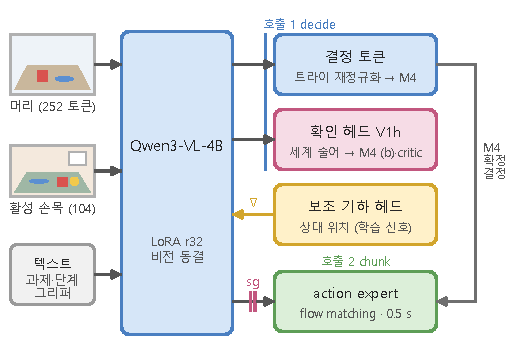
\includegraphics[width=\linewidth]{figures/model.pdf}
\caption{\textbf{조이스틱 VLA.} 머리 카메라와 활성 팔 손목 카메라를 원본 해상도 다중 이미지로 넣고, 과제 문장·구간 의도 줄·그리퍼 상태·움직임 줄을 붙인다. 결정 스텝마다 두 번 부른다. \textbf{decide}: 한 번의 순전파로 결정 토큰의 보기 확률(\cref{eq:trie})과 확인 헤드 V1h의 세계 쪽 술어를 낸다. 보조 기하 헤드는 시뮬 특권 상태의 상대 위치를 예측하는 학습 신호이며 실행 때는 쓰지 않는다. \textbf{chunk}: 행동 전문가가 기울기 차단(KI) 뒤의 문맥 은닉 상태를 읽고, M4가 확정한 결정을 조건으로 0.5\,s 청크를 낸다. 전문가가 결정을 따르게 하는 것은 먼 구간 반사실 분기 학습이 맡는다(\cref{sec:vla}). 영상 탑은 얼리고, 헤드 크기와 손실 가중치는 \tentative{가정값}이다.}
\label{fig:model}
\end{figure}

\paragraph{조이스틱 VLA.} 백본은 Qwen3-VL-4B~\cite{qwen3vl2025}이고 영상 탑은 얼린다. 머리 카메라와 지금 움직이는 팔의 손목 카메라를 원본 해상도 다중 이미지로 넣고, 상태 텍스트(과제 문장, 그리퍼 상태, 거친 움직임 줄)를 붙인다. 모델은 문장을 생성하지 않는다. 질문 $q$의 보기 이름들을 토큰 트라이로 만들고, 갈림 노드 $n$마다 자식 토큰끼리만 softmax를 취해 곱한다.
\begin{equation}
  \tilde p(o\mid x,q) \;=\; \prod_{n\in\mathrm{path}(o)} \frac{\exp z_{n,c(n,o)}}{\sum_{c\in\mathrm{child}(n)}\exp z_{n,c}}.
  \label{eq:trie}
\end{equation}
결정 호출은 약 0.33\,s 간격으로 겹쳐 나가며, 확정 규칙 M4가 호출 사이 합의와 실행 뒤 측정(T1, V1h)을 결합해 확정한다(부록 \cref{sec:supp_m4}). 행동 전문가는 백본 은닉 상태 $h$를 교차 주의로 읽고, 확정된(상위 목표와 섞인) 결정을 조건으로 청크 $A$를 낸다.
\begin{equation}
  \mathcal{L}_{\text{act}} = \mathbb{E}_{\tau,\epsilon}\bigl\|\,v_\theta(A^\tau, \tau \mid \mathrm{sg}[h]) - (\epsilon - A)\,\bigr\|^2,\quad A^\tau = \tau\epsilon + (1-\tau)A.
  \label{eq:fm}
\end{equation}
KI~\cite{kinsulate2025}대로 전문가에서 백본으로 가는 기울기를 막는다($\mathrm{sg}$).

\paragraph{결정이 실행을 조종하게.} 섞은 결정이 실행을 바꾸려면 전문가가 결정을 실제로 따라야 한다. 학습 데이터에서 결정은 영상만 보면 정해지므로 전문가는 결정 토큰을 볼 이유가 없고, 실제로 학습 없이 조건만 바꿔 잰 진단에서 강제 방향을 우연 수준으로만 따랐다. 그래서 물체에서 먼 구간의 스냅샷에 강제 방향과 그 방향의 직선 청크를 짝지은 \emph{반사실 분기}를 흐름 정합 배치에 섞는다. 실데이터 레시피는 분기 75\%다(\cref{sec:evidence_stage2}).

\paragraph{VLA 학습 계획 (\tentative{보류}).} 결정 항, 행동 항, 보조 기하 항, 확인 헤드 항을 함께 학습한다. 층을 다시 넣게 되면 끝-끝 학습을 더한다. KI 절연은 유지한 채 백본이 이산 행동 토큰도 예측하게 하고, 전문가의 조건을 정답 결정에서 예측 결정으로 옮기는 교과를 쓴다. 결합 고리 안의 DAgger와 교란 학습은 ``상위 목표에서 온 결정'' 입력에 맞춰 다시 정의한다(목표가 낡거나 틀린 경우 포함). 상위는 1단계에서 학습한 것을 그대로 쓴다.
